\documentclass{article}
\usepackage{graphicx} % Required for inserting images
\usepackage[margin=1in]{geometry}
\usepackage{listings}
\usepackage{xcolor}
\usepackage{amsmath}
\usepackage[hidelinks]{hyperref}
\usepackage{amssymb}

\title{MATH 20D Review}
\author{Kevin Jacob}
\date{Fall 2025}

\begin{document}

\maketitle

\newpage

\section*{Table of Contents}
\begin{enumerate}
    \item \hyperref[sec:overview]{Differential Equation Overview}
    \item \hyperref[sec:first]{First Order Differential Equations}
    \begin{itemize}
        \item \hyperref[sec:flinear]{First Order Linear Differential Equations}
        \item \hyperref[sec:fintegratefactor]{Method of Integrating Factors}
        \item \hyperref[sec:fseperable]{First Order Seperable Differential Equations}
        \item \hyperref[sec:uniqueness]{Existence and Uniqueness of Solutions}
        \item \hyperref[sec:fautonomous]{Autonomous Differential Equations}
        \item \hyperref[sec:fexact]{Exact Differential Equations}
    \end{itemize}
\end{enumerate}
\newpage
\section{Differential Equation Overview}
\label{sec:overview}
\subsection{Direction Fields}
With a differential equation in the form $y'(x)=f(x,y)$, this is a grid of line segments on the xy-plane obtained by drawing a short line segment at each $(x,y)$ whose slope is $f(x,y)$
\begin{center}
    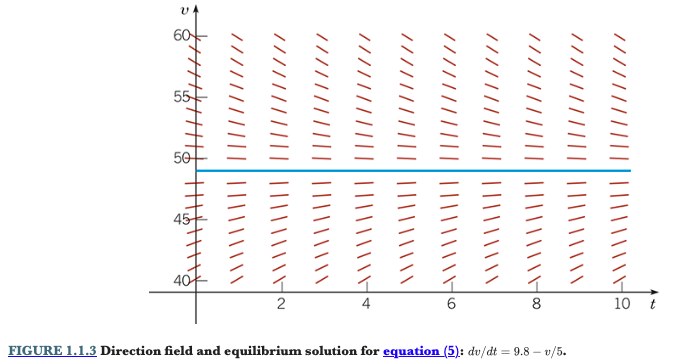
\includegraphics[scale=0.5]{directionField.png}
\end{center}
\subsection{Differential Equation Example}
$\frac{dp}{dt}=0.5p-450$\\
$\frac{dp}{dt}=\frac{p-900}{2}$\\
$\frac{dp/dt}{p-900}=\frac{1}{2}$\\
$\frac{d}{dt}\ln \vert p-900\vert=\frac{1}{2}$\\
$\ln \vert p-900\vert = \frac{t}{2}+C$\\
$\vert p-900\vert=e^{t/2 + C}=e^Ce^{t/2}$\\
$p-900=\pm e^Ce^{t/2}$\\
$p=900+ce^{t/2}$ where $c=\pm e^C$\\
\newline
Suppose $p(0)=850$, then we get $850=900+c$ so $c=-50$. The solution will then be $p=900-50e^{t/2}$. $p(0)=850$ is an example of an \textbf{initial condition}, and the differential equation with the initial condition forms an \textbf{initial value problem}. In the case where we don't have an initial value, we can end up with an expression called the \textbf{general solution} which is an infinite family of \textbf{integral curves} where each interval curve is associated with a particular value of $c$.
\subsection{Classifying Differential Equations}
\subsubsection{Linear vs. Non-Linear}
The ordinary differential equation is said to be linear if it can be written as $F(x,y(x),y'(x),\dots,y^{(n)}(x))=0$ where $F$ is a linear function of the variables $y,y',\dots,y^{(n)}$. The general linear ordinary differential equation of order $n$ is
\begin{center}
    $a_m(x)y^{(n)}(x)+\dots+a_1(x)y'(x)+a_0(x)y(x)=0$
\end{center}
An example of a non-linear differential equation is $y(x)y'(x)=4y(x)$
\newpage
\subsubsection{Ordinary vs. Partial Differential Equations}
Ordinary differential equations are equations where the unknown function depends only on one variable. In the second case where the function depends on more than one variable the derivatives are partial derivatives and the equation is called a partial differential equation.\\
Ordinary Differential Equation Example: $\frac{dy(x)}{dx}+4y(x)=0$\\
Partial Differential Equation Example: $\frac{\partial y(x,t)}{\partial x}+4y(x,t)=0$
\subsubsection{System of Differential Equations}
When more than one unknown functions are present. Below is an example of the predator-prey system used for ecological modeling
\begin{center}
    $\frac{dx}{dt}=ax-\alpha xy$\\
    $\frac{dy}{dx}=-cy+\gamma xy$\\
    $a,\alpha, c, \gamma$ are predator constants and this is a system of non-linear ordinary differential equations
\end{center}
\subsubsection{Order of a Differential Equation}
The order of a differential equation if the order of the highest derivative that appears in the equation.\\
2nd order differential equation: $y''(x)+6y'(x)=35[y(x)]^2$
\subsubsection{Classification Examples}
\begin{itemize}
    \item $y'(x)=0$: first order linear ODE
    \item $[y''(x)]^2+4=0$: second order non-linear ODE
    \item $\frac{\partial^2u]}{\partial x^2}-\frac{1}{x^2}\frac{\partial u}{\partial t}=0$: second order linear PDE
    \item $\frac{dp(t)}{dt}=\frac{p(t)}{2}-4$: first order linear ODE
    \item $y'(x)=-4y(x)$: first order linear ODE
    \item $y''(t)=-9.8$: second order linear ODE
    \item $[y'''(x)]^4+[y''(x)]^6=sin([y(x)]^2-y'(x))$: third order non-linear ODE
\end{itemize}
\section{First Order Differential Equations}
\label{sec:first}
\subsection{First Order Linear Differential Equations}
\label{sec:flinear}
$y\sim y'(t)\dots a\sim a(t), b\sim b(t), c\sim c(t)$ where $a(t)y'(t)+b(t)=c(t)$ is the simplest DE one can solve\\
\textbf{Examples}
\begin{enumerate}
    \item $y'(t)=2t$\\
    $\frac{dy(t)}{dt}=2t$\\
    Integrate both sides with respect to $t$\\
    $\int\frac{dy(t)}{dt}dt=\int2tdt\rightarrow y(t)=t^2+c$ (general solution)\\
    When given initial condition $y(0)=1$, the unique solution to the initial value problem is $y(t)=t^2+1$
    \item $y(t)y'(t)=t$ (non-linear)\\
    $2y(t)y'(t)=2t$\\
    $\frac{d}{dt}[y(t)]^2=2t$\\
    Integrate both sides with respect to $t$\\
    $\int\frac{d}{dt}[y(t)]^2dt=\int 2tdt$\\
    $[y(t)]^2=t^2+c$\\
    $y(t)=\sqrt{t^2+c}$\\
    If $c\geq 0$ then $y(t)$ is defined for $t\in\mathbb{R}$. If $c=-1$ the $y(t)$ only defined when $\vert t \vert\geq 1$.
    \item $(4+t^2)\frac{dy(t)}{dt}+2ty=4t$\\
    $(4+t^2)\frac{dy(t)}{dt}+\frac{d}{dt}(t^2+4)y(t)=4t$\\
    $\frac{d}{dt}[(4+t^2)y(t)]=4t$\\
    Integrate both sides with respect to $t$\\
    $\int\frac{d}{dt}[(4+t^2)y(t)]dt=\int 4tdt$\\
    $(4+t^2)y(t)=2t^2+c$\\
    $y(t)=\frac{2t^2}{4+t^2}+\frac{c}{4+t^2}$ (general solution)
\end{enumerate}
\subsection{Method of Integrating Factors}
\label{sec:fintegratefactor}
If we have a first order linear ODE ($\frac{dy}{dt}+p(t)y(t)=g(t)$), we can multiply the equation by a certain function $\mu(t)$ which will make the differential equation immediately integrable by using the product rule for derivatives.\\
\textbf{Example:} $\frac{dy(t)}{dt}+2y(t)=\frac{e^t}{3}$\\
We need to multiply both functions by integrating factor $\mu(t)$\\
$\mu(t)\frac{dy(t)}{dt}+2\mu(t)y(t)=\frac{e^t}{3}\mu(t)$\\
Chose $\mu(t)$ so that $LHS=\frac{d}{dt}(\mu(t)y(t))$\\
$\frac{d}{dt}(\mu(t)y(t))=\mu(t)\frac{dy(t)}{dt}+y(t)\frac{d\mu(t)}{dt}$\\
$\frac{d\mu(t)}{dt}=2\mu(t)$\\
$\frac{1}{\mu(t)}\frac{d\mu(t)}{dt}=2$\\
$\frac{d}{dt}\ln\vert \mu(t)\vert=2$\\
$\int\frac{d}{dt}\ln\vert \mu(t)\vert dt=\int 2dt$\\
$\ln\vert \mu(t)\vert =2t+c$\\
$\mu(t)=e^{2t}, c=0$\\
Plug in $\mu(t)$\\
$e^{2t}\frac{dy(t)}{dt}+2e^{2t}y(t)=\frac{e^t}{3}\cdot e^{2t}$\\
$\frac{d}{dt}(e^{2t}y(t))=\frac{e^{3t}}{3}$\\
$e^{2t}y(t)=\frac{e^{3t}}{9}+c$\\
$y(t)=\frac{e^t}{9}+ce^{-2t}$ (General Solution)\\
\newline
\textbf{Find Integrating Factor}\\
Given the first order linear ODE in the form $\frac{dy}{dt}+p(t)y(t)=g(t)$, the integrating factor is $\mu(t)=e^{\int p(t)dt}$.\\
\textbf{Example:} $y'(t)+\frac{1}{t}y(t)=2t$ on $t>0$\\
$p(t)=\frac{1}{t}$\hspace*{0.5in}$g(t)=2t$\\
$\mu(t)=e^{\int p(t)dt}=e^{\int\frac{1}{t}dt}=e^{\ln t}=t$\\
$\mu(t)[y'(t)+\frac{1}{t}y(t)]=2t\mu(t)$\\
$\frac{d}{dt}(\mu(t)y(t))=2t\mu(t)$\\
$\frac{d}{dt}(ty(t))=2t^3$\\
$ty(t)=\frac{2t^3}{3}+c$\\
$y(t)=\frac{2t^2}{3}+\frac{c}{t}$ (general solution)
\subsection{First Order Seperable Differential Equations}
\label{sec:fseperable}
Suppose we have a differentiable equation in the form $y'(x)=f(x,y(x))$ (can be non-linear) that we can write as $M(x,y)+N(x,y)y'(x)=0$. When $M$ is a function of $x$ only and $N$ is a function of $y$ only the equation becomes $M(x)+N(y)y'(x)=0$ which is said to be separable. \\
\textbf{Examples}
\begin{enumerate}
    \item $y'(x)=\frac{x^2}{1-y^2}$\\
    $-x^2+(1-y^2)y'=0$\\
    $\int-x^2dx+\int(1-y^2)y'dx=\int0dx$\\
    $-\int x^2dx+\int(1-y^2)dy=\int0dx$\\
    $-\frac{x^3}{3}+y-\frac{y^3}{3}=c$
    \item $y'(x)=\frac{3x^2+4}{2y-4}$, $y(0)=1$\\
    $-(3x^2+4)+(2y(x)-4)y'(x)=0$\\
    $-\int(3x^2+4)dx+\int(2y-4)dy=\int0dx$\\
    $-x^3-4x+y^2-4y=c$\\
    Sub in $y(0)=1$ which gives $-0^3-4(0)+1^2-4(1)=c\rightarrow c=-3$\\
    $y^2-4y=x^3+4x-3$\\
    $y^2-4y+4=x^3+4x-3+4$\\
    $(y-2)^2=x^3+4x+1$\\
    $y-2=\pm\sqrt{x^3+4x+1}$\\
    $y(x)=2\pm\sqrt{x^3+4x+1}$\\
    $y(x)=2-\sqrt{x^3+4x+1}$ satisfies the initial condition and is the explicit solution
    \item $y'(x)=\frac{xy^3}{\sqrt{1+x^2}}$, $y(0)=1$, and find largest possible interval on which solution is defined\\
    $\frac{y'}{y^3}=\frac{x}{\sqrt{1+x^2}}$\\
    $\int\frac{1}{y^3}dy=\in\frac{x}{\sqrt{1+x^2}}dx$\\
    $-\frac{1}{2y^2}=\sqrt{1+x^2}+c$\\
    Sub in $y(0)=1$ which gives $-\frac{1}{2}=1+c\rightarrow c=-\frac{3}{2}$\\
    $-\frac{1}{2y^2}=-\frac{3}{2}+\sqrt{1+x^2}\rightarrow y=\pm\frac{1}{\sqrt{3-2\sqrt{1+x^2}}}$\\
    Take $y=\frac{1}{\sqrt{3-2\sqrt{1+x^2}}}$ based on initial condition which is defined when $3-2\sqrt{1+x^2}>0$ or $\vert x\vert<\frac{\sqrt{3}}{2}$
    \item $y'(x)=3t^2(y-4)$, $y(0)=y_0$ where $y_0=4$ or $y_0=8$
    \begin{itemize}
        \item $y_0=4$\\
        $y(t)=4$ is a possible solution (check for constant solutions)
        \item $y_0=8$\\
        $\frac{y'(t)}{y(t)-4}=3t^2$ ($y(t)\neq4$ to avoid dividing by zero)\\
        $\int\frac{y'(t)}{y(t)-4}dt=\int3t^2dt$\\
        $\int\frac{1}{y-4}dy=t^3+c$\\
        $\ln\vert y(t)-4\vert=t^3+c$\\
        $\vert y(t)-4\vert=e^{t^3+c}$\\
        $\pm(y(t)-4)=e^{t^3+c}$\\
        Sub in $y(0)=8$ which gives $\pm(8-4)=e^{0+c}$ and since $e^c$ is not negative, $e^c=4\rightarrow c=\ln4$\\
        $y(t)-4=e^{t^3+\ln4}\rightarrow y(t)=4+e^{t^3+\ln4}$
    \end{itemize}
\end{enumerate}
\subsection{Existence and Uniqueness of Solutions}
\label{sec:uniqueness}
\subsubsection{Existence and Uniqueness of solutions to 1st order linear ODEs (Theorem 2.4.1)}
Let $p$ and $g$ be continuous functions defined on the interval $I=(\alpha,\beta)$. Then for all $y_0$, the IVP
\begin{center}
    $y'+py=g$\\
    $y(t_0)=y_0$
\end{center}
has a unique solution $\Phi$ defined on $(\alpha,\beta)$.\\
\newpage
\textbf{Proof}
Using method of integrating factors and fundamental theorem of calculus, suppose that $f$ is a continuous function on $[a,b]$ and $F$ satisfies $F'(t)=f(t)$ for all $t$ in $(a,b)$. Then for only $a\leq t\leq b$, $F(t)-F(a)=\int_a^tf(s)ds$.\\
$\mu(t)(y'(t)+p(t)y(t))=g(t)\mu(t)\rightarrow\begin{cases}
    \frac{d}{dt}(\mu(t) y(t))=g(t)\mu(t)\\
    y(t_0)=y_0
\end{cases}$\\
Treat $\mu(t) y(t)$ as $F$ and $g(t)\mu(t)$ as $f$\\
$F(t)-F(t_0)=\int_{t_0}^tf(s)ds$\\
$\mu(t) y(t)-\mu(t_0) y(t_0)=\int_{t_0}^tf(s)ds$\\
$\mu(t) y(t)=\int_{t_0}^tf(s)ds+y_0$\\
$y(t)=\frac{1}{\mu(t)}[\int_{t_0}^tf(s)ds+y_0]$\\
\newline
\textbf{Example}\\
$ty'(t)+2y=4t^2$\\
If $t\neq 0$\\
$y'(t)+\frac{2}{t}y=4t$\\
$p(t)=\frac{2}{t}$ and $g(t)=4t$, so $p$ and $g$ are both continuous on $(0,\infty)\cup(-\infty,0)$. According to the theorem the initial value problem $y'+\frac{2}{t}y=4t$, $y(1)=2$ has a unique solution defined on $(0,\infty)$. $\Phi(t)=t^2+\frac{1}{t^2}$.
\subsubsection{Existence and Uniqueness of solutions to 1st order non-linear ODE (Theorem 2.4.2)}
Let $f$, $\frac{\partial f}{\partial y}$ be continuous on a rectangle $(\alpha,\beta)\times(\gamma,\delta)$ in the ty-plane containing $(t_0,y_0)$. Then there is some interval $(t_0-h,t_0+h)$ contained in $(\alpha,\beta)$ such that the IVP $y(t)=f(t,y(t))$, $y(t_0)=y_0$ has a unique solution defined on $(t_0-h,t_0+h)$\\
$y'=-p(t)y+g(t)\rightarrow f(t,y)=-p(t)y+g(t)$\\
If $f,\frac{\partial f}{\partial y}$ are continuous, $\frac{\partial f}{\partial y}=-p(t)$. $\frac{\partial f}{\partial y}$ is a continuous function of $y,t$ which implies $p(t)$ is continuous and if $f(t,y)+p(t)y=g(t)$ then $g(t)$ is continuous in $t$.\\ 
\textbf{Examples}
\begin{enumerate}
    \item $y'(x)=\frac{3x^3+4x+2}{2(y-1)}$\\
    $f(x,y)=\frac{3x^2+4x+2}{2(y-1)}$\hspace*{0.5in}$\frac{\partial f}{\partial y}=\frac{-(3x^2+4x+2)}{2(y-1)^2}$
    \begin{itemize}
        \item $y(0)=-1$\\
        Both $f,\frac{\partial f}{\partial y}$ are continuous on $(-\infty,\infty)\times(-2,0)$ containing the point $(0,-1)$ and based on theorem 2.4.2 there is a unique solution on $(-h,h)$\\
        $y'(x)=\frac{3x^2+4x+2}{2(y-1)}$\\
        $\int 2(y-1)y'(x)dx=\int(3x^2+4x+2)dx$\\
        $y^2-2y=x^3+2x^2+2x+c$\\
        Sub in $y(0)=-1$ we get $(-1)^2-2(-1)=c\rightarrow c=3$\\
        $y^2-2y=x^3+2x^2+2x+3\rightarrow y=1\pm\sqrt{x^3+2x^2+2x+4}$\\
        $y=1-\sqrt{x^3+2x^2+2x+4}$ is unique solution that satisfies $y(0)=-1$
        \item $y(0)=1$\\
        Both $f,\frac{\partial f}{\partial y}$ are discontinuous on every rectangle containing $(0,1)$ so theorem 2.4.2 doesn't apply to the initial value problem\\
        $y=1\pm\sqrt{x^3+2x^2+2x+4}$ both satisfy $y(0)=1$ so we have 2 solutions
    \end{itemize}
    \item $y'(x)=(y(x))^{1/3}$, $y(0)=0$\\
    $f(x,y)=y^{1/3}$\hspace*{0.5in}$\frac{\partial f}{\partial y}=\frac{1}{3}y^{-2/3}$\\
    No matter how small of a rectangle we take, $\frac{\partial f}{\partial y}$ is still not continuous at $(0,0)$ so theorem 2.4.2 fails\\
    $y'(x)=(y(x))^{1/3}$\\
    $\frac{y'(x)dx}{[y(x)]^{1/3}}=dx$\\
    $\int\frac{1}{y^{1/3}}dy=\int dx$\\
    $\frac{2}{3}y^{2/3}=x+c$\\
    $y=[\frac{2}{3}(x+c)]^{3/2}$\\
    Sub in $y(0)=0$, we get $c=0$\\
    $y(x)=\pm(\frac{2}{3}x)^{3/2}$ are both solutions (square root)\\
    $y(x)=0$ is also a solution
    \item $y'=y^2$, $y(0)=y_0$\\
    $f(x,y)=y^2$\hspace*{0.5in}$\frac{\partial f}{\partial x}=2y$\\
    Both $f,\frac{\partial f}{\partial x}$ are continuous on entire xy-plane\\
    $y'=y^2$\\
    $\frac{y'}{y^2}dx=dx$\\
    $\int\frac{1}{y^2}dy=\int dx$\\
    $-\frac{1}{y}=x+c$\\
    Sub in $y(0)=y_0$, we get $c=-\frac{1}{y_0}$\\
    $y(x)=\frac{y_0}{1-y_0}$ is the solution which is not defined when $x=\frac{1}{y_0}$ so the solution is defined on the interval $(-\frac{1}{t_0},\frac{1}{t_0})$
\end{enumerate}
\subsection{Autonomous Differential Equations}
\label{sec:fautonomous}
An autonomous differential equation is a differntial equation of the form
\begin{center}
    $y'=f(y)$
\end{center}
We don't need to explicitly solve the differential equation to understand the long term behavior of solutions\\
\textbf{logistic model:} $y'=r(1-\frac{y}{k})y$
\begin{itemize}
    \item $r$ is the intrinsic rate of growth/decline
    \item $k$ is the saturation level or environmental converging capacity
\end{itemize}
\textbf{Step 1:} sketch $y$ vs $f(y)$
The y-axis is called the \textbf{phase line} and the dots at $y=0$ and $y=k$ are the critical points (or equilibrium solutions). The arrows indicate that $y$ is increasing whenever $0<y<k$ and that $y$ is decreasing when $y>k$.
\begin{center}
    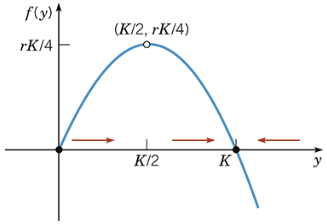
\includegraphics[scale=0.6]{yvsfy.png}
\end{center}
\textbf{Step 2:} Plot $y$ vs $t$ (solution curves) and include phase line along $y$ axis.\\
If $f,\frac{df}{dy}$ have the same sign, $y(t)$ is concave up and if they have opposite signs the graph is concave down.\\
$f(y)=r(1-\frac{y}{k})y$\hspace*{0.25in}$f(y)=0$ if $y=k,0$\\
$f'(y)=r(1-\frac{2y}{k})$\hspace*{0.25in}$f'(y)=0$ if $y=\frac{k}{2}$\\
Concave up $0<t<\frac{k}{2}$ and $k<t<\infty$ | concave down $\frac{k}{2}<t<k$
\begin{center}
    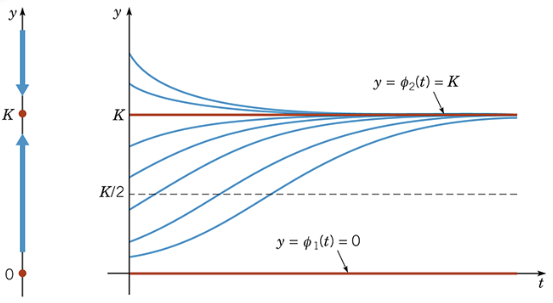
\includegraphics[scale=0.6]{yvst.png}
\end{center}
\textbf{Equilibrium Stability}
\begin{itemize}
    \item Stable Equilibrium: $\Phi t(t)=a$ is a stable equilibrium solution if any nearby solutions asymptotically approach $y=a$ as $t\rightarrow\infty$
    \item Unstable Equilibrium: $\Phi (t)=a$ is a unstable equilibrium if solutions diverge from $y=a$ as $t\rightarrow\infty$
    \item Semi-Stable Equilibrium: $\Phi (t)=a$ is a semi-stable equilibrium if solutions on one side asymptotically approach $y=a$ and solutions on another side diverge as $t\rightarrow\infty$
\end{itemize}
\subsection{Exact Differential Equations}
\label{sec:fexact}
An exact differential equation is a differential equation in the form
\begin{center}
   $\frac{\partial\Psi(x,y)}{\partial x}+\frac{\partial\Psi(x,y)}{\partial y}y'(x)=0$ 
\end{center}
$\Psi(x,y)$ is a function of $x$ and $y$ where $y$ is a function of $x$. $\Psi(x,y(x))=c$ is an implicit solution\\
\newline
\textbf{Check if ODE is exact (theorem 2.6.1)}\\
Let $M,N,\frac{\partial M}{\partial y},\frac{\partial N}{\partial x}$ be continuous on a rectangular region $(\alpha,\beta)\times(\gamma,\delta)$. Then the equation $M(x,y)+n(x,y)y'(x)=0$ is exact \textit{if and only if} $\frac{\partial M}{\partial y}=\frac{\partial N}{\partial x}$ at all points in the rectangle.\\
\newline
\textbf{Examples}
\begin{enumerate}
    \item $(x^2\cos y-y\sin x)+(x\sin y+y\cos x)y'=0$\\
    $M(x,y)=x^2\cos y-y\sin x$\hspace*{0.5in}$N(x,y)=x\sin y+y\cos x$\\
    $\frac{\partial M}{\partial y}=-x^2\sin y-\sin x$\hspace*{0.5in}$\frac{\partial N}{\partial x}=\sin y-y\sin x$\\
    Since $\frac{\partial M}{\partial y}\neq\frac{\partial N}{\partial x}$, the differential equation is not exact
    \item $\frac{2xy}{x^2+1}-2x-(2-\ln(x^2+1))y'=0$\\
    $M(x,y)=\frac{2xy}{x^2+1}-2x$\hspace*{0.5in}$N(x,y)=-(2-\ln(x^2+1))$\\
    $\frac{\partial M}{\partial y}=\frac{2x}{x^2+1}$\hspace*{0.5in}$\frac{\partial N}{\partial x}=\frac{2x}{x^2+1}$\\
    Since $\frac{\partial M}{\partial y}=\frac{\partial N}{\partial x}$, the differential equation is exact so there is a function $\Psi(x,y)$ such that $\frac{\partial\Psi}{\partial x}=M(x,y)$ and $\frac{\partial\Psi}{\partial y}=N(x,y)$
\end{enumerate}
\textbf{Find $\Psi$}
\newpage
\textit{Based on the example above}\\
$\frac{\partial\Psi}{\partial x}=\frac{2xy}{x^2+1}-2x$ (treat $y$ as constant)\\
$\Psi(x,y)=\int(\frac{2xy}{x^2+1}-2x)dx=y\ln(x^2+1)-x^2+h(y)$\\
$\Psi(x,y)=y\ln(x^2+1)-x^2+h(y)$\\
To find $h(y)$ we use the equation $\frac{\partial\Psi}{\partial y}=N(x,y)$\\
$\ln(x^2+1)+h'(y)=-2(2-\ln(x^2+1))$\\
$h'(y)=-2$\\
$h(y)=-2y+c$\\
$\Psi(x,y)=y\ln(x^2+1)-x^2-2y+c$\\
Solution $\Psi(x,y)=c'$ (implicitly defines $y$ as function of $x$)\\
$y\ln(x^2+1)-x^2-2y+c=c'\rightarrow y\ln(x^2+1)-x^2-2y=\overset{\sim}{c}$\\
$\Phi(x)\ln(x^2+1)-x^2-2\Phi(x)=\overset{\sim}{c}\rightarrow \Psi(x,\Phi(x))=C$
\end{document}
